\documentclass[9pt,twocolumn,letterpaper]{article}

\usepackage[english]{babel}
\usepackage[utf8]{inputenc}
\usepackage[T1]{fontenc}
\usepackage[letterpaper,top=0.68in,bottom=0.68in,left=0.64in,right=0.64in]{geometry}
\usepackage{amsmath,amssymb,amsfonts}
\usepackage{booktabs}
\usepackage{multirow}
\usepackage{array}
\usepackage{graphicx}
\usepackage{tikz}
\usepackage{pgfplots}
\usepackage{subcaption}
\usepackage[font=small,skip=2pt]{caption}
\usepackage{xcolor}
\usepackage{hyperref}
\usetikzlibrary{positioning}

\pgfplotsset{compat=1.18}
\setlength{\columnsep}{0.18in}
\renewcommand{\arraystretch}{0.94}
\setlength{\textfloatsep}{8pt plus 1pt minus 2pt}
\setlength{\floatsep}{6pt plus 1pt minus 2pt}
\setlength{\intextsep}{6pt plus 1pt minus 2pt}
\setlength{\dbltextfloatsep}{7pt plus 1pt minus 2pt}
\setlength{\abovecaptionskip}{2pt}
\setlength{\belowcaptionskip}{0pt}
\setlength{\abovedisplayskip}{5pt}
\setlength{\belowdisplayskip}{5pt}
\setlength{\abovedisplayshortskip}{4pt}
\setlength{\belowdisplayshortskip}{4pt}

\title{
\usefont{OT1}{bch}{b}{n}
\normalfont \small \textsc{Cross-Corpus Speech Emotion Recognition Study} \\ [4pt]
\huge Representation, Alignment, and Classifier Effects in Cross-Corpus Speech Emotion Recognition \\
}

\usepackage{authblk}

\author[1]{Pranav Singh}
\author[1]{Prashant Singh}
\author[1]{Akshat Bawa}
\affil[1]{\footnotesize Indian Institute of Technology (IIT), Ropar}
\date{}

\begin{document}
\maketitle

\begin{abstract}
Cross-corpus speech emotion recognition (SER) remains difficult because models trained on one corpus often degrade sharply on another with different speakers, recording conditions, elicitation styles, and label distributions. We present an empirical study using three self-supervised speech backbones (HuBERT, wav2vec 2.0, and WavLM), a hybrid SSL+MFCC representation, three alignment settings (none, CORAL, and MMD), three blending strategies (none, scalar, and group-adaptive alignment), and four classifier families (logistic regression, SVM, MLP, and a lightweight Transformer). Experiments cover in-domain and full cross-domain evaluation across RAVDESS, CREMA-D, and IEMOCAP with pair-specific shared label spaces. Results indicate a pronounced in-domain to cross-domain gap, substantial transfer asymmetry, and strong sensitivity to representation choice. HuBERT is strongest on average; alignment yields dataset-dependent gains; blending is not uniformly beneficial; and simple classifiers remain competitive. The main contribution is a systematic comparison clarifying how SSL representations, hybrid fusion, alignment, and classifier choice interact under domain shift.
\end{abstract}

\noindent
Keywords: speech emotion recognition, cross-corpus generalization, domain adaptation, self-supervised speech representation, empirical evaluation

\section{Introduction}
Speech emotion recognition has matured considerably within individual corpora, yet robust generalization across datasets remains unresolved. Emotional cues are entangled with speaker identity, recording conditions, elicitation protocols, annotation practice, and corpus-specific lexical content, so systems that perform well within a corpus often deteriorate across corpora \cite{schuller2010cross}. This gap remains a major barrier to practical SER deployment.

The study considers three widely used corpora: RAVDESS \cite{livingstone2018ryerson}, CREMA-D \cite{cao2014crema}, and IEMOCAP \cite{busso2008iemocap}. They differ in speaking style, recording setup, speaker population, and label inventory. RAVDESS and CREMA-D share a six-class space, whereas experiments involving IEMOCAP use the five-class overlap. This enables both in-domain speaker-independent evaluation and controlled cross-domain transfer.

Recent self-supervised speech models have substantially improved SER front ends, but it remains unclear which representations are most stable under domain shift. wav2vec 2.0 \cite{baevski2020wav2vec}, HuBERT \cite{hsu2021hubert}, and WavLM \cite{chen2022wavlm} are strong candidates with different pretraining objectives and inductive biases. Representation quality may alter downstream transfer more than small classifier changes. Likewise, feature alignment is a common remedy for corpus mismatch, but methods such as CORAL \cite{sun2016deep} and MMD \cite{gretton2012kernel} need not help uniformly.

These considerations motivate a broader empirical study. Rather than focusing on one backbone or alignment family, we compare multiple SSL representations, alignment strategies, a hybrid SSL+MFCC design, and classifiers ranging from linear baselines to lightweight nonlinear models. We also test blending mechanisms that interpolate between original and aligned features. The study asks how much backbone choice matters, whether alignment consistently improves cross-corpus SER, whether hybrid fusion remains useful alongside SSL features, and whether more complex classifiers are preferable under domain shift.

The experiments reveal three broad patterns: a large in-domain to cross-domain gap, marked transfer asymmetry, and strong dependence of alignment and blending gains on the source-target pair and backbone. The aim is therefore a clear empirical account of cross-corpus behavior rather than a claim of universal superiority.

\section{Materials \& Methods}
\subsection{Datasets and preprocessing}
RAVDESS \cite{livingstone2018ryerson}, CREMA-D \cite{cao2014crema}, and IEMOCAP \cite{busso2008iemocap} were evaluated under speaker-independent splits. Audio preprocessing was fixed for all experiments and consisted of mono conversion, resampling to $16$ kHz, and peak amplitude normalization. Label spaces were matched per source-target pair. RAVDESS and CREMA-D experiments use six shared classes (angry, disgust, fear, happy, neutral, and sad), while experiments involving IEMOCAP use the five-class intersection (angry, fear, happy, neutral, and sad).

\subsection{Backbone representations}
The system extracts utterance-level embeddings from three self-supervised speech encoders: wav2vec 2.0 Base \cite{baevski2020wav2vec}, HuBERT Base \cite{hsu2021hubert}, and WavLM Base \cite{chen2022wavlm}. For each backbone, frame-level embeddings $h_t \in \mathbb{R}^{D}$ are mean pooled:
\begin{equation}
z = \frac{1}{T}\sum_{t=1}^{T} h_t.
\end{equation}
The pooled representation $z$ is the SSL input to the alignment and blending stages. All comparisons use the same pooling rule so that performance differences can be attributed to backbone, alignment, blending, or classifier choice rather than temporal aggregation.

\subsection{MFCC acoustic features}
In parallel with the SSL branch, we extract Mel-frequency cepstral coefficients (MFCCs) from the same waveform. MFCCs summarize the short-term spectral envelope on the Mel scale and remain useful in SER because they retain information related to timbre, articulation, and coarse prosodic variation. The acoustic branch uses $13$ base coefficients with first- and second-order differences, yielding a $39$-dimensional frame-level representation that is mean pooled to an utterance-level vector $m \in \mathbb{R}^{39}$. This handcrafted branch is retained to test whether low-level acoustic cues still complement SSL features under corpus shift, not to assume guaranteed gains.

\subsection{Pipeline overview}
Figure \ref{fig:pipeline} summarizes the modular two-branch pipeline. In the SSL branch, a selected backbone produces pooled embeddings that may be aligned and blended. In the acoustic branch, MFCC features are extracted and pooled without alignment. Alignment is applied only to the SSL branch to isolate domain matching in the learned representation space while keeping the handcrafted branch fixed. The final representation is
\begin{equation}
X_{\mathrm{hybrid}} = \left[ X_{\mathrm{SSL}}^{\mathrm{final}} \; ; \; X_{\mathrm{MFCC}} \right],
\end{equation}
where $X_{\mathrm{SSL}}^{\mathrm{final}}$ denotes the aligned or blended SSL features and $X_{\mathrm{MFCC}}$ the pooled MFCC vector. This enables comparison of backbones, alignment, hybrid fusion, and classifiers under one protocol.

\begin{figure}[t]
\centering
\resizebox{\columnwidth}{!}{
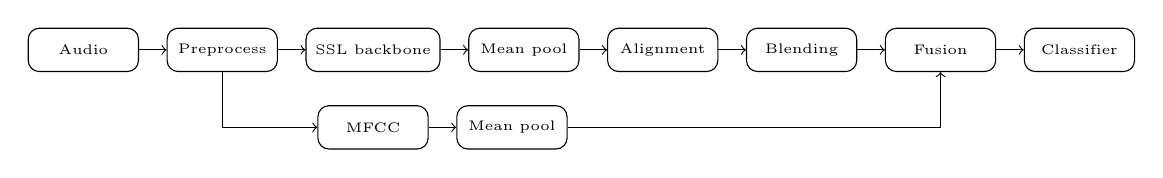
\begin{tikzpicture}[
node distance=0.42cm and 0.35cm,
every node/.style={font=\tiny},
box/.style={draw, rounded corners, align=center, minimum width=1.4cm, minimum height=0.55cm}
]
\node[box] (audio) {Audio};
\node[box, right=of audio] (prep) {Preprocess};
\node[box, right=of prep] (ssl) {SSL backbone};
\node[box, below=of ssl] (mfcc) {MFCC};
\node[box, right=of ssl] (pool) {Mean pool};
\node[box, right=of mfcc] (mfccpool) {Mean pool};
\node[box, right=of pool] (align) {Alignment};
\node[box, right=of align] (blend) {Blending};
\node[box, right=of blend] (fuse) {Fusion};
\node[box, right=of fuse] (clf) {Classifier};
\draw[->] (audio) -- (prep);
\draw[->] (prep) -- (ssl);
\draw[->] (prep) |- (mfcc);
\draw[->] (ssl) -- (pool);
\draw[->] (mfcc) -- (mfccpool);
\draw[->] (pool) -- (align);
\draw[->] (align) -- (blend);
\draw[->] (blend) -- (fuse);
\draw[->] (mfccpool) -| (fuse);
\draw[->] (fuse) -- (clf);
\end{tikzpicture}
}
\caption{Hybrid pipeline: pooled SSL features undergo optional alignment and blending, then concatenate with pooled MFCC features before classification. Alignment is applied only to the SSL branch.}
\label{fig:pipeline}
\end{figure}

\subsection{Alignment methods}
Let $X_s$ and $X_t$ denote source and target feature matrices after pooling. Three alignment settings are considered.

\textbf{None.} Features are used without explicit domain adaptation.

\textbf{CORAL.} CORAL matches second-order statistics by whitening the source covariance and recoloring it with the target covariance \cite{sun2016deep}:
\begin{equation}
X_s^{\mathrm{coral}} = (X_s - \mu_s) C_s^{-1/2} C_t^{1/2} + \mu_t,
\end{equation}
where $\mu_s$ and $\mu_t$ are source and target means and $C_s$, $C_t$ are regularized covariance matrices.

\textbf{MMD.} Maximum Mean Discrepancy (MMD) reduces the discrepancy between source and target feature distributions in reproducing-kernel Hilbert space \cite{gretton2012kernel}, yielding an aligned representation $X_s^{\mathrm{mmd}}$ without relying only on second-order matching.

\subsection{Blending strategies}
Alignment can be followed by blending between the original representation $X^{\mathrm{orig}}$ and the aligned representation $X^{\mathrm{align}}$. Three blending modes are evaluated.

\textbf{None.} The aligned representation is passed directly to the classifier if alignment is enabled; otherwise the original representation is used.

\textbf{Scalar blending.} A single interpolation coefficient $\alpha$ is applied to all dimensions:
\begin{equation}
X^{\mathrm{final}} = \alpha X^{\mathrm{align}} + (1-\alpha)X^{\mathrm{orig}}.
\end{equation}

\textbf{Group-adaptive alignment (GAA).} Feature dimensions are clustered into groups, and each group receives its own interpolation coefficient. If $\mathcal{I}_g$ denotes the index set for group $g$, then
\begin{equation}
X^{\mathrm{final}}[:,\mathcal{I}_g] =
\alpha_g X^{\mathrm{align}}[:,\mathcal{I}_g] +
(1-\alpha_g) X^{\mathrm{orig}}[:,\mathcal{I}_g].
\end{equation}
This reduces adaptation rigidity without fully independent per-dimension coefficients.

\subsection{Classifiers}
Four classifier families are compared. Logistic regression is the linear baseline; SVM provides a class-balanced kernel method; MLP is a lightweight nonlinear feed-forward model. The Transformer baseline is a compact two-layer encoder applied to reshaped pooled utterance-level features. It uses a small per-token hidden dimension and a single attention head per layer to remain computationally comparable to the other nonlinear baselines. The aim is controlled comparison, not maximal architectural scale.

\subsection{Evaluation protocol}
The complete grid spans three backbones, three alignment settings, three blending settings, four classifiers, and all nine source-target combinations among RAVDESS, CREMA-D, and IEMOCAP, yielding $972$ runs. In-domain runs correspond to $src=tgt$; all others are cross-domain. Accuracy and macro-F1 are reported, with macro-F1 as the primary metric because class imbalance and class collapse are common under cross-corpus transfer. Nonlinear classifiers, including the Transformer, were trained under the same budget: Adam, learning rate $10^{-3}$, fixed mini-batches, and eight epochs. No separate early stopping was used.

\section{Results}
The strongest cross-domain configuration achieved macro-F1 $0.4111$ on RAVDESS $\rightarrow$ CREMA-D using HuBERT, MMD, GAA, and logistic regression. This shows that the modular pipeline can work well in favorable transfer settings even though average cross-corpus performance remains much lower. Results are therefore presented in two stages: best-case configurations first, then aggregate trends.

\begin{table*}[t]
\centering
\caption{Top cross-domain configurations by macro-F1.}
\label{tab:best_configs}
\footnotesize
\setlength{\tabcolsep}{3pt}
\begin{tabular}{lccccc}
\toprule
Source $\rightarrow$ Target & Backbone & Alignment & Blending & Classifier & Macro-F1 \\
\midrule
RAVDESS $\rightarrow$ CREMA-D & HuBERT & MMD & GAA & LogReg & 0.4111 \\
RAVDESS $\rightarrow$ CREMA-D & HuBERT & MMD & Scalar ($\alpha=0.5$) & LogReg & 0.3995 \\
RAVDESS $\rightarrow$ CREMA-D & HuBERT & MMD & None & MLP & 0.3775 \\
RAVDESS $\rightarrow$ CREMA-D & HuBERT & MMD & None & LogReg & 0.3730 \\
CREMA-D $\rightarrow$ RAVDESS & HuBERT & MMD & GAA & SVM & 0.3715 \\
RAVDESS $\rightarrow$ CREMA-D & HuBERT & CORAL & GAA & SVM & 0.3658 \\
RAVDESS $\rightarrow$ CREMA-D & HuBERT & None & None & LogReg & 0.3635 \\
RAVDESS $\rightarrow$ CREMA-D & HuBERT & MMD & GAA & MLP & 0.3633 \\
\bottomrule
\end{tabular}
\end{table*}

Table \ref{tab:best_configs} shows that the strongest results are concentrated in a small subset of transfer directions, especially RAVDESS $\rightarrow$ CREMA-D, and are dominated by HuBERT-based representations. It also shows that strong performance depends on combinations of backbone, alignment, blending, and classifier rather than any single component.

The full matrix nevertheless confirms that cross-corpus SER is dominated by domain shift. Averaged over all settings, in-domain macro-F1 is $0.4384$, whereas cross-domain macro-F1 drops to $0.1579$. This gap persists across all backbones and classifier families. Table \ref{tab:backbone_alignment} summarizes backbone and alignment effects, Table \ref{tab:blending} blending effects in aligned settings, Table \ref{tab:classifier} classifier averages, and Table \ref{tab:domain_gap} the backbone-specific domain gap.

\begin{table}[t]
\centering
\caption{Mean cross-domain macro-F1 by backbone and alignment.}
\label{tab:backbone_alignment}
\scriptsize
\setlength{\tabcolsep}{2.5pt}
\begin{tabular}{lccc}
\toprule
Backbone & None & CORAL & MMD \\
\midrule
HuBERT & 0.1473 & 0.2005 & 0.1964 \\
wav2vec 2.0 & 0.1127 & 0.1553 & 0.1561 \\
WavLM & 0.1159 & 0.1718 & 0.1652 \\
\bottomrule
\end{tabular}
\end{table}

\begin{table}[t]
\centering
\caption{Mean cross-domain macro-F1 for blending in aligned settings.}
\label{tab:blending}
\scriptsize
\setlength{\tabcolsep}{2.5pt}
\begin{tabular}{lcc}
\toprule
Blending & Mean macro-F1 & Relative rank \\
\midrule
None & 0.1852 & 1 \\
GAA & 0.1804 & 2 \\
Scalar & 0.1572 & 3 \\
\bottomrule
\end{tabular}
\end{table}

\begin{table}[t]
\centering
\caption{Mean macro-F1 by classifier.}
\label{tab:classifier}
\scriptsize
\setlength{\tabcolsep}{2.5pt}
\begin{tabular}{lcc}
\toprule
Classifier & In-dom. & Cross-dom. \\
\midrule
LogReg & 0.5926 & 0.1731 \\
SVM & 0.5628 & 0.1539 \\
MLP & 0.4716 & 0.1882 \\
Transformer & 0.4366 & 0.1636 \\
\bottomrule
\end{tabular}
\end{table}

\begin{table}[t]
\centering
\caption{Backbone-specific mean macro-F1.}
\label{tab:domain_gap}
\scriptsize
\setlength{\tabcolsep}{2.5pt}
\begin{tabular}{lccc}
\toprule
Backbone & In-domain & Cross-domain & Gap \\
\midrule
HuBERT & 0.4566 & 0.1814 & 0.2752 \\
wav2vec 2.0 & 0.4083 & 0.1414 & 0.2669 \\
WavLM & 0.4503 & 0.1510 & 0.2993 \\
\bottomrule
\end{tabular}
\end{table}

Several trends emerge in the full grid. Table \ref{tab:backbone_alignment} shows that HuBERT is strongest on average under cross-domain evaluation, with mean macro-F1 of $0.1473$ without alignment and about $0.20$ after CORAL or MMD. WavLM is intermediate, while wav2vec 2.0 is weakest on average. The ranking is not uniform for every source-target pair, but backbone choice exerts a consistent effect.

Alignment helps on average, but gains are uneven. For all backbones, CORAL and MMD improve mean cross-domain macro-F1 relative to no alignment. Their difference is modest, and the better method depends on the transfer pair. For example, mean F1 for RAVDESS $\rightarrow$ CREMA-D rises from $0.1388$ with no alignment to $0.2211$ with CORAL and $0.2232$ with MMD, whereas IEMOCAP $\rightarrow$ RAVDESS remains low under all three settings ($0.0700$, $0.0893$, and $0.0918$). Alignment therefore helps in some settings without resolving severe mismatch in others.

Blending requires similarly cautious interpretation. Table \ref{tab:blending} shows that, within aligned settings, no blending has the highest average cross-domain macro-F1 ($0.1852$), GAA is close ($0.1804$), and scalar blending is lower ($0.1572$). Yet GAA appears in several of the strongest individual configurations in Table \ref{tab:best_configs}, including the overall best result. Its value is therefore transfer-dependent rather than universal.

Classifier behavior also varies with regime. Table \ref{tab:classifier} shows that logistic regression is strongest on average in-domain and remains highly competitive cross-domain. MLP achieves the highest average cross-domain macro-F1 ($0.1882$), but its advantage over LogReg is modest, and the best cross-domain configurations are distributed across LogReg, MLP, and SVM. The Transformer is competitive in several settings without a consistent average advantage. Overall, representation quality and transfer compatibility matter more than classifier complexity alone.

Transfer asymmetry is visible throughout the pairwise results. Mean macro-F1 for RAVDESS $\rightarrow$ CREMA-D is $0.1944$, whereas CREMA-D $\rightarrow$ RAVDESS is $0.1653$. The asymmetry is larger for RAVDESS and IEMOCAP ($0.1424$ versus $0.0837$), while CREMA-D and IEMOCAP remain asymmetric as well ($0.2034$ versus $0.1583$). Domain shift is therefore directional, not symmetric.

\subsection{Comparison with Prior Work}
Recent SER studies increasingly rely on self-supervised representations, transfer learning, and domain adaptation. Direct numerical comparison remains imperfect because datasets, emotion inventories, splits, adaptation budgets, and metrics differ substantially. Table \ref{tab:prior_work} is therefore contextual rather than strictly equivalent. Its role is to situate the paper within recent literature while clarifying that the present contribution is a controlled study of representation, alignment, hybrid fusion, and classifier interactions rather than a single aggressively tuned transfer system.

\begin{table*}[t]
\centering
\caption{Contextual comparison with prior work. Protocols and metrics differ across studies.}
\label{tab:prior_work}
\scriptsize
\setlength{\tabcolsep}{2pt}
\begin{tabular}{p{1.9cm}p{1.6cm}p{2.7cm}p{2.1cm}p{1.0cm}p{3.2cm}}
\toprule
Method & Backbone & Adaptation / Strategy & Datasets & Metric & Reported performance \\
\midrule
Pastor et al. \cite{pastor2023cross} & HuBERT, WavLM & Cross-corpus training extension & EmoDB, RAVDESS, CREMA-D, IEMOCAP & UAR & WavLM + CNN-SA reports 66.90\% UAR on IEMOCAP and 70.92\% on RAVDESS. \\
Naderi and Nasersharif \cite{naderi2023cross} & wav2vec 2.0 + prosody & Attention fusion + TL with 20\% target speakers & IEMOCAP $\rightarrow$ EmoDB, others & Acc. & AFTL reports 92.45\% accuracy on EmoDB. \\
Fu et al. \cite{fu2023cross} & DDAE acoustic features & Multi-task + LMMD subdomain adaptation & Berlin, eNTERFACE, CASIA & WAR & Average WAR improves by 1.89\%--10.07\% over comparison models. \\
Latif et al. \cite{latif2023self} & SSL adversarial features & Dual-discriminator adaptation + synthetic augmentation & IEMOCAP, MSP-IMPROV, EMO-DB, FAU-AIBO, others & UAR & sADDi reports 48.61\% UAR for IEMOCAP $\rightarrow$ MSP-IMPROV and 58.3\% for IEMOCAP $\rightarrow$ FAU-AIBO. \\
Jafari et al. \cite{jafari2025feature} & DistilHuBERT & Feature- and classifier-level adaptation & EMODB, IEMOCAP, ShEMO & Acc. & Best DistilHuBERT reaches 92.01\% accuracy on EMODB from ShEMO source. \\
Ma et al. \cite{ma2024emobox} & SSL benchmark incl. HuBERT, WavLM, wav2vec 2.0, Whisper & Balanced cross-corpus benchmark & IEMOCAP, MELD, RAVDESS, SAVEE & Acc. & Whisper large v3 averages 52.01\%; HuBERT base 40.34\%; WavLM base 38.28\%. \\
Ours & HuBERT / WavLM + MFCC hybrid & Controlled comparison of SSL+MFCC fusion, CORAL/MMD, GAA, classifiers & RAVDESS, CREMA-D, IEMOCAP & Macro-F1 & Best cross-domain result: HuBERT + MMD + GAA + LogReg on RAVDESS $\rightarrow$ CREMA-D with 0.4111 macro-F1. \\
\bottomrule
\end{tabular}
\end{table*}

Table \ref{tab:prior_work} also clarifies the paper's emphasis. Several prior systems optimize narrower transfer settings through larger architectures, supervised or partially supervised fine-tuning, adversarial adaptation, or attention-based fusion \cite{naderi2023cross,latif2023self,jafari2025feature}, whereas benchmark-oriented work emphasizes broad PTM coverage and standardized splits \cite{ma2024emobox}. The present paper sits between these directions: it uses a lightweight modular pipeline to study interactions among backbone choice, SSL+MFCC fusion, alignment, blending, and classifier complexity. Performance is competitive in some transfer pairs, but the broader pattern remains severe and unstable domain shift.

Figure \ref{fig:cmats} illustrates these effects with confusion matrices. The strongest cross-domain case, a strong in-domain case, and the two transfer directions under the same HuBERT + MMD + GAA + logistic regression setting show that alignment reduces mismatch without eliminating corpus-specific confusion structure or directional asymmetry.

\begin{figure*}[t]
\centering
\begin{subfigure}[t]{0.24\textwidth}
\centering
\includegraphics[width=\textwidth]{ravdess_crema_hubert_mmd_gaa_logreg.png}
\caption{R$\rightarrow$C best cross-domain.}
\end{subfigure}\hfill
\begin{subfigure}[t]{0.24\textwidth}
\centering
\includegraphics[width=\textwidth]{ravdess_ravdess_wavlm_coral_gaa_logreg.png}
\caption{R$\rightarrow$R strong in-domain.}
\end{subfigure}\hfill
\begin{subfigure}[t]{0.24\textwidth}
\centering
\includegraphics[width=\textwidth]{ravdess_crema_hubert_mmd_gaa_logreg.png}
\caption{R$\rightarrow$C direction.}
\end{subfigure}\hfill
\begin{subfigure}[t]{0.24\textwidth}
\centering
\includegraphics[width=\textwidth]{crema_ravdess_hubert_mmd_gaa_logreg.png}
\caption{C$\rightarrow$R direction.}
\end{subfigure}
\caption{Representative confusion matrices from stored results. The same aligned setting behaves differently across transfer directions.}
\label{fig:cmats}
\end{figure*}

\section{Discussion}
The most stable conclusion is that domain shift remains the dominant challenge in cross-corpus SER. The in-domain to cross-domain gap is large for every backbone and classifier family, and even the best cross-domain settings remain well below the strongest in-domain ones.

Backbone choice is a major source of variation. HuBERT is strongest on average, WavLM is generally second, and wav2vec 2.0 is weakest in the aggregate cross-domain comparison. Although not absolute for every pair, this ordering is consistent enough to make representation choice one of the most consequential design decisions.

Alignment methods provide inconsistent gains rather than a universal remedy. CORAL and MMD improve cross-domain mean macro-F1 on average, yet their effects vary by source-target pair. In particular, IEMOCAP $\rightarrow$ RAVDESS remains difficult under every alignment setting. Feature matching can therefore help when mismatch is amenable to distribution alignment, but not when it is more structural.

The blending results reinforce this caution. Neither scalar blending nor GAA is uniformly beneficial. GAA contributes to some of the best individual configurations, but its mean cross-domain performance is slightly below the no-blending alternative in aligned settings, while scalar blending is weaker on average. Blending can help, but its value is conditional on source-target pair, backbone, and classifier.

The hybrid representation should be interpreted similarly. The design combines aligned SSL features with an unaligned MFCC branch because handcrafted acoustic cues may complement pooled SSL embeddings under corpus shift. Qualitative comparison suggests that hybrid fusion can stabilize some transfer settings, but the effect is modest and dataset-dependent rather than universally dominant.

Classifier complexity also fails to produce a simple hierarchy. MLP achieves the highest average cross-domain score, but logistic regression is competitive, produces some of the strongest individual transfer results, and surpasses SVM and Transformer on average under cross-domain evaluation. Complexity is therefore not sufficient to overcome domain shift when the representation-transfer interaction is unfavorable.

One possible explanation for the Transformer outcome is that the downstream classifier operates on pooled utterance-level embeddings rather than full frame sequences. Because pooling already compresses much of the temporal structure, an additional attention head may have limited opportunity to exploit sequence relationships beyond what the SSL representation already encodes. This interpretation remains tentative. A related limitation is that the Transformer was intentionally lightweight; larger sequence-level architectures or less aggressive pooling may behave differently.

Finally, the experiments show persistent asymmetry. Transfer from RAVDESS to CREMA-D is stronger than the reverse direction, and analogous asymmetries appear in the pairs involving IEMOCAP. Cross-corpus SER should therefore not be summarized only by undirected corpus similarity; $A \rightarrow B$ and $B \rightarrow A$ are distinct empirical problems.

\section*{Conclusions}
This paper presented a systematic study of cross-corpus SER across three SSL backbones, a hybrid SSL+MFCC pipeline, three alignment settings, three blending strategies, four classifiers, and full source-target evaluation on RAVDESS, CREMA-D, and IEMOCAP. HuBERT is the most reliable backbone on average; alignment often helps but inconsistently; blending is transfer-dependent; and simple classifiers remain competitive. More broadly, performance depends on the interaction among representation, alignment, classifier, and transfer direction rather than any single adaptation mechanism. Future progress is therefore likely to come from understanding when a particular combination is appropriate for a given source-target pair.

\section*{Acknowledgements}
The authors acknowledge the public release of the RAVDESS, CREMA-D, and IEMOCAP corpora, which made this comparative study possible.

\begin{thebibliography}{99}

\bibitem{schuller2010cross}
B. Schuller, B. Vlasenko, F. Eyben, G. Rigoll, and A. Wendemuth,
``Cross-corpus acoustic emotion recognition: Variances and strategies,''
\textit{IEEE Transactions on Affective Computing}, vol. 1, no. 2, pp. 119--131, 2010.

\bibitem{livingstone2018ryerson}
S. R. Livingstone and F. A. Russo,
``The Ryerson Audio-Visual Database of Emotional Speech and Song (RAVDESS): A dynamic, multimodal set of facial and vocal expressions in North American English,''
\textit{PLOS ONE}, vol. 13, no. 5, p. e0196391, 2018.

\bibitem{cao2014crema}
H. Cao, D. G. Cooper, M. K. Keutmann, R. C. Gur, A. Nenkova, and R. Verma,
``CREMA-D: Crowd-sourced emotional multimodal actors dataset,''
\textit{IEEE Transactions on Affective Computing}, vol. 5, no. 4, pp. 377--390, 2014.

\bibitem{busso2008iemocap}
C. Busso, M. Bulut, C.-C. Lee, A. Kazemzadeh, E. Mower, S. Kim, J. Chang, S. Lee, and S. Narayanan,
``IEMOCAP: Interactive emotional dyadic motion capture database,''
\textit{Language Resources and Evaluation}, vol. 42, no. 4, pp. 335--359, 2008.

\bibitem{pastor2023cross}
M. A. Pastor, D. Ribas, A. Ortega, A. Miguel, and E. Lleida,
``Cross-corpus training strategy for speech emotion recognition using self-supervised representations,''
\textit{Applied Sciences}, vol. 13, no. 16, p. 9062, 2023.

\bibitem{naderi2023cross}
N. Naderi and B. Nasersharif,
``Cross corpus speech emotion recognition using transfer learning and attention-based fusion of Wav2Vec2 and prosody features,''
\textit{Knowledge-Based Systems}, vol. 277, p. 110814, 2023.

\bibitem{fu2023cross}
H. Fu, Z. Zhuang, Y. Wang, C. Huang, and W. Duan,
``Cross-corpus speech emotion recognition based on multi-task learning and subdomain adaptation,''
\textit{Entropy}, vol. 25, no. 1, p. 124, 2023.

\bibitem{latif2023self}
S. Latif, R. Rana, S. Khalifa, R. Jurdak, and B. Schuller,
``Self supervised adversarial domain adaptation for cross-corpus and cross-language speech emotion recognition,''
\textit{IEEE Transactions on Affective Computing}, vol. 14, no. 3, pp. 1912--1926, 2023.

\bibitem{jafari2025feature}
M. Jafari, F. Shahin, and A. Alavi,
``Feature and classifier-level domain adaptation in DistilHuBERT for cross-corpus speech emotion recognition,''
\textit{Computers in Biology and Medicine}, vol. 187, p. 110510, 2025.

\bibitem{ma2024emobox}
Z. Ma, M. Chen, H. Zhang, Z. Zheng, W. Chen, X. Li, J. Ye, X. Chen, and T. Hain,
``EmoBox: Multilingual multi-corpus speech emotion recognition toolkit and benchmark,''
in \textit{Proc. Interspeech}, 2024, pp. 1580--1584.

\bibitem{baevski2020wav2vec}
A. Baevski, H. Zhou, A. Mohamed, and M. Auli,
``wav2vec 2.0: A framework for self-supervised learning of speech representations,''
in \textit{Advances in Neural Information Processing Systems}, 2020, pp. 12449--12460.

\bibitem{hsu2021hubert}
W.-N. Hsu, B. Bolte, Y.-H. H. Tsai, K. Lakhotia, R. Salakhutdinov, and A. Mohamed,
``HuBERT: Self-supervised speech representation learning by masked prediction of hidden units,''
\textit{IEEE/ACM Transactions on Audio, Speech, and Language Processing}, vol. 29, pp. 3451--3460, 2021.

\bibitem{chen2022wavlm}
S. Chen, C. Wang, Z. Chen, Y. Wu, S. Liu, J. Li, N. Wang, T. Zhou, and F. Wei,
``WavLM: Large-scale self-supervised pre-training for full stack speech processing,''
\textit{IEEE Journal of Selected Topics in Signal Processing}, vol. 16, no. 6, pp. 1505--1518, 2022.

\bibitem{sun2016deep}
B. Sun and K. Saenko,
``Deep CORAL: Correlation alignment for deep domain adaptation,''
in \textit{European Conference on Computer Vision Workshops}, 2016, pp. 443--450.

\bibitem{gretton2012kernel}
A. Gretton, K. M. Borgwardt, M. J. Rasch, B. Sch\"olkopf, and A. Smola,
``A kernel two-sample test,''
\textit{Journal of Machine Learning Research}, vol. 13, pp. 723--773, 2012.

\bibitem{w2vprosody2023}
M. Ploszaj, P. Tarnowski, and P. W. Jedrzejczak,
``Cross-corpus speech emotion recognition using transfer learning and attention-based fusion of wav2vec2 and prosody features,''
\textit{Knowledge-Based Systems}, vol. 275, p. 110676, 2023.

\bibitem{li2023cross}
Y. Li, J. Wu, X. Liu, and H. Meng,
``Cross-corpus speech emotion recognition based on multi-task learning and subdomain adaptation,''
\textit{Entropy}, vol. 25, no. 1, p. 124, 2023.

\end{thebibliography}

\end{document}
